% The Editorial Office Requirements for the Table of Contents cause a significant problem
%in Latex if there is only one Appendix. The Appendix is no longer labeled "A" in the TOC
%but has the word "APPENDIX" placed in front of the title of the Appendix. This can be done
%without issue IF nothing needs to be numbered by LaTeX in the Appendix. Unfortunately, most of the time
%something needs to be numbered in that single Appendix. For this reason we have included the IFTHENELSE switch
%found in this document and at the beginning of AppendixA. We assume that if you have any appendices, that you have more than one. However, you DO only have one appendix DO NOT USE THIS FILE!!!!!!!!!!!!!!!!!!!!!!!
%
% OneSingleAppendix.tex has all the settings needed to adjust for a single appendix
% you will have a major problem with your TOC if you use this file with a single appendix!!!!!

%
% Comment (or delete) all of the \input{AppendixB} commands except those you are using.
%Then open the AppendixA.tex file and continue there.

%you can add/substract individual appendices through by using the /include{appendix'X'}
% and creating/deleting the appropriate files
\appendix %
%\clearpage%

\addtocontents{toc}{\protect\addvspace{10pt}\noindent{APPENDIX} \protect\hfill\par}{}


% % % % % % % If you have a single appendix, you should be using appendix1.tex
% % % % % % % NOT this file

\chapter{Orthonormal Basis Functions and Mercer's Theorem}
\label{a:mercers_theorem}

Given an RKHS $\clH$, it is useful to understand the set of functions that belong to the Hilbert space. This can be studied using Mercer's theorem \cite{merrus09}. Mercer's theorem forms the connection between the theory of reproducing kernels and integral operators. 
Consider the integral operator (Hilbert-Schmidt operator) $L_K:L^2_\measure(x) \to L^2_\measure(x)$ defined by,
\begin{equation}
(L_K f)(x) = \int_\state \Kern(x,t) f(t) d\measure(t)
\end{equation}
where $\measure$ is a finite Borel measure and $\state$ is a compact set.
The linear map $L_K^{1/2}$, which denotes the square root of $L_K$ is a Hilbert isomorphism between $L^2_{\measure}(\state)$ and $\clH$ as illustrated in \Fig{fig:rkhs_isomorphism}. 

\begin{figure}[htbp]
	\centering
	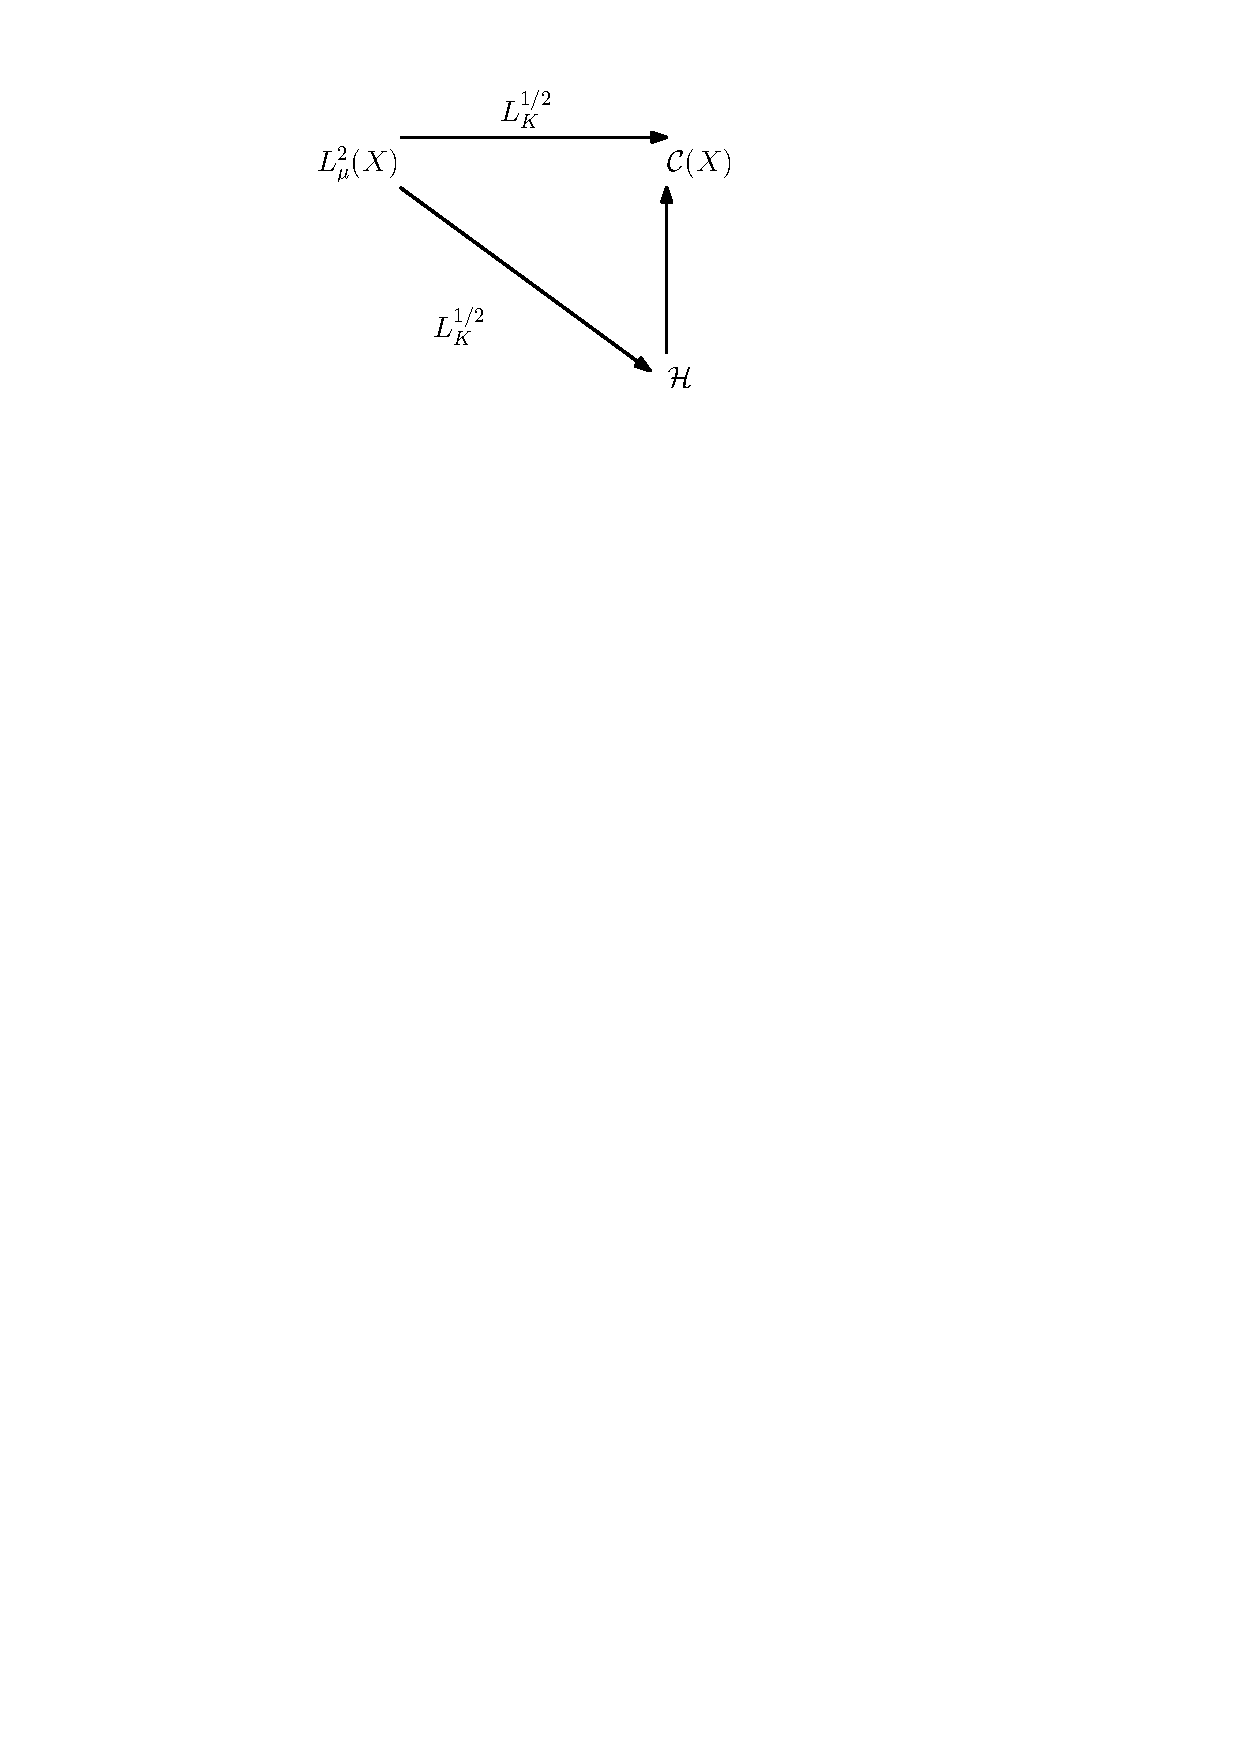
\includegraphics[width=3in]{images/Chap3_RKHS_isomorphism}
	\caption{Diagram illustrating the isomorphic transformations between $\clH$ and $L^2_\measure$.}
	\label{fig:rkhs_isomorphism}
\end{figure}

% $L_{K,C}$ emphasizes that the target is $\mathcal{C}(\state)$ and $I_K$ denotes the inclusion. If $\Kern$ is $\mathcal{C}^\infty$, then $I_K$ is compact. \anand{Gaussian kernel is $\mathcal{C}^\infty$}
$L_K$ is a self-adjoint, compact operator with eigenvalues $\reg_1 \geq \reg_2 \geq \cdots \geq 0$, with the corresponding normalized eigenfunctions $\{\phi_n\}_{n=1}^\infty$ forming an orthonormal basis for $L^2_\measure(\state)$. Mercer's theorem states that 
\begin{equation}
\Kern(x,x') = \sum_{n=1}^\infty \reg_n \phi_n(x) \phi_n(x'),
\end{equation}
where the series converges absolutely for each $x,x' \in \state$. The set $\{\sqrt{\reg_n}\phi_n\}_{n=1}^\infty$ forms an orthonormal basis for $\clH$. However, finding an eigenfunction feature representation for a kernel is challenging, except in special cases. 
 %
\chapter{Properties of the Gaussian Kernel -  RKHS}%
\label{a:gaussian_rkhs}

Of the many kernels being used, Gaussian kernel is the most widely used and often gives the best performance \cite{min10}. The study of the properties of the Gaussan kernel has received a lot of attention \cite{stehussco06, min10,micchaxuzha06}. The Gaussian kernel is a translation-invariant kernel given by,
\begin{equation}
\Kern_{\epsilon}(x,x') := \exp(-\|x - x'\|^2/ 4\epsilon) \qquad \forall x,x' \in \state,
\end{equation}
where $\epsilon$ is a parameter that defines the width of the kernel. An illustration of the Gaussian kernel for $\epsilon = 0.125$ and the corresponding Fourier transform is given in \Fig{fig:gaussian_kernel}. It may be seen that the Fourier transform decays exponentially fast for large values of $\omega$. The lack of high frequency components in the Gaussian kernel indicates that the functions belonging to the induced RKHS are smooth.  
\begin{figure}[htbp]
	\centering
	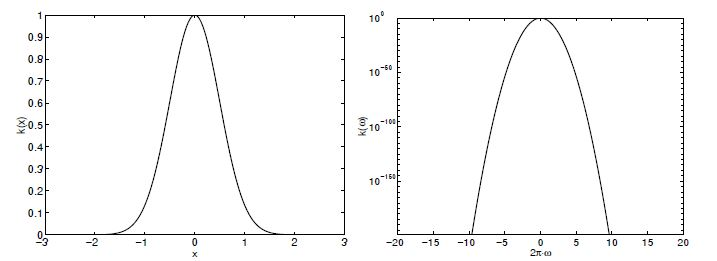
\includegraphics[width=6in]{images/Chap3_Gaussian_kernel}
	\caption{Gaussian kernel with $\epsilon = 0.125$ and its Fourier transform \cite{schsmo01}.}
	\label{fig:gaussian_kernel}
\end{figure}

Steinwart et al. in \cite{stehussco06} tries to answer questions like - which functions are contained in the RKHS induced by the Gaussian kernel, how the corresponding norms can be computed, and how the RKHS of different widths correlate to each other. 
In particular, RKHS of Gaussian kernels always have countable orthonormal bases. Theorem 3 of the paper gives the orthonormal basis functions for $\clH$ defined by the Gaussian kernel $\Kern_\epsilon$. It states that for $\epsilon >0$ and $n \in \mathbb{N}_0 := \mathbb{N} \cup \{0\}$, the sequence of functions $\{\phi_n : \Re \to \Re\}$ defined by,
\begin{equation}
\phi_n(x) := \sqrt{\frac{1}{(2\epsilon)^n n!}}x^n \exp(-x^2/4\epsilon).
\end{equation}
is an orthonormal basis for $\clH$.

Minh in \cite{min10} gives several properties of the RKHS induced by Gaussian kernels. Theorem 1 of the paper states that the RKHS $\clH$ induced by the standard Gaussian kernel is infinite dimensional, i.e. dim($\clH$) = $\infty$ and 
\begin{equation}
\clH := \Bigl\{ f = \exp(-x^2/4\epsilon) \sum_{n=0}^\infty w_n x^n: \|f\|^2_\clH = \sum_{k=0}^\infty (2\epsilon)^k k! \sum_{n=0}^k w_n^2 <\infty \Bigr\}
\end{equation}
Some of the salient properties of the Gaussian kernel RKHS are summarized below: 
\begin{arabnum}
	\item $\clH$ induced by the standard Gaussian kernel does not contain any polynomial on $\state$, including the non-zero constant function. 
	
	\item If $\state$ is compact, $\clH$ induced by the Gaussian kernel is dense in the space of $\mathcal{C}(\state)$ of continuous functions on $\state$.
	This means that given a continuous function $h(x)$, for all $\varepsilon >0$, we can find a function $g(x) \in \clH$ such that 
	\begin{equation}
	\|h(x) - g(x)\|_\infty \leq \epsilon \qquad \forall x \in \state
	\end{equation} 
	\item Let $\Kern_{\epsilon}(x,x') = \exp(-\frac{\|x-x'\|^2}{4\epsilon})$. The Hilbert space $\clH_\epsilon$ induced by $\Kern_\epsilon$ on $\state$ contains the function $\exp(-\frac{c \|x\|^2} {4 \epsilon})$ if and only if $0<c <2$. For example, $\exp(-\frac{\|x\|^2}{2 \epsilon}) \in \clH_{\epsilon/2}$, but  $\exp(-\frac{\|x\|^2}{2 \epsilon}) \notin \clH_{\epsilon}$. As $c=0$ is excluded, it validates the first property that constant functions do not belong to $\clH$.
	
	\item The functions in $\clH$ that are smooth are not necessarily integrable, as $\clH \notin L^1(\Re^n)$ for any $\epsilon >0$.  This implies that $L^1$ norm optimization or regularization is infeasible in $\clH$. This could still be done on subsets of finite linear combinations of the basis functions.
	
	
	\item Partial derivatives of the Gaussian kernel denoted as $\frac{\partial^n}{\partial x^n} \Kern_x \in \clH$. As a corollary, it can be shown that $t^n \Kern_x(t)\in\clH$. Additionally, for any polynomial $p(t)$, $p(t) \Kern_x(t) \in \clH$. An expression for the Hilbert space norm for kernel derivative of any order $d$ is also provided in \cite{min10}. 
\end{arabnum}

The paper by Michelli et al. \cite{micchaxuzha06} sets out to identify kernels with universal approximating property, i.e. given any compact set $\state$, any function $f \in \mathcal{C}(\state)$, there is a function $g \in \clH$ such that $\| f - g\|_{\infty} \leq \varepsilon$ holds for any $\varepsilon > 0$. Thus for any choice of compact set $\state$, the space $\clH$ is dense in $\mathcal{C}(\state)$ in the maximum norm. A kernel that satisfies this property is called the universal kernel. The paper discusses the characterization of universal kernels in terms of feature map representation of the kernel $\Kern$. It provides necessary and sufficient condition for $\Kern$ to have the universal approximation property in terms of its features. Under conditions provided in Theorem 17 of the paper, the standard Gaussian kernel is shown to be universal. 
 %
\chapter{Proof of Representer Theorem \Theorem{theorem:rep_theorem}}%
\label{a:reptheorem}

\begin{proof}
	From the definition of the RKHS $\clH$, any $f$ of the form:
	\[
	f \eqdef \sum_{i=1}^N  
	\beta_i \Kern(x_i,\cdot),
	\]
	is in $\clH$. 	
	Denote the linear subspace of $\clH$ made up of all such functions $f$ that are finite linear combinations of the kernel functions centered at $x_i$,
	\[
	\clH_\shortparallel := \Bigl\{f \in \clH\, |\, f = \sum_{i=1}^N  \beta_i \Kern(x_i,\cdot) \Bigr\},
	\]
	where $N$ ranges over $\mathbb{Z}_+$, and  each $\beta_i \in \Re$ for each $i$. Denote by $\clH_{\perp}$, the subspace of $\clH$ orthogonal to $\clH_\shortparallel$:
	\[
	\clH_\perp : = \{ \tilf \in \clH\,| \, \langle \tilf , f \rangle_\clH = 0 ,\, \forall f \in \clH_\shortparallel \}
	\]
	We can see that every $f \in \clH$ can be uniquely decomposed into a component lying within $\clH_\shortparallel$, denoted by $f_\shortparallel$ and a component lying within $\clH_\perp$, denoted by $f_\perp$.
	The $\clH$-norm can be written as,
	\[
	\Omega(\|f\|_\clH) = \Omega( \|f_\shortparallel + f_\perp\|_\clH) =\Omega( \sqrt{\|f_\shortparallel\|^2_\clH + \|f_\perp\|^2_\clH})  \geq \Omega(\|f_\shortparallel\|_\clH)
	\]
	The inequality is obtained from the fact that $\|f_\perp\|_\clH \geq 0$ and the function $\Omega(\cdot)$ is a strict monotone.
	This implies that the regularization term in \eqref{e:erm_rkhs} is minimized if $f$ lies in the subspace $\clH_\shortparallel$.
	Additionally, using reproducing property of the kernel $\Kern$,
	\[
	\begin{aligned}
	f(x_i) & =  \langle f \, , \Kern(x_i,.) \rangle_\clH\\
	&  = \langle f_\shortparallel\, , \Kern(x_i,.) \rangle_\clH + \langle f_\perp \, , \Kern(x_i,.) \rangle_\clH \\
	&  = \langle f_\shortparallel\, , K(x_i,.) \rangle_\clH \\
	&  = f_\shortparallel(x_i).
	\end{aligned}
	\]
	Therefore,
	\[
	L(x_i, f(x_i)) = L(x_i, f_\shortparallel(x_i))
	\]
	The empirical error term depends only on the component $f_\shortparallel$. Hence, the regularized objective function is minimized if $f_\reg^*$ lies within $\clH_\shortparallel$ and takes the form,
	\[
	f_\reg^*(x) = \sum_{i=1}^N  \beta_i^*  \Kern(x_i, x)
	\]
	This concludes the proof. 
\end{proof} %
\chapter{Generalization Error Bounds for least-squares regression on RKHS }%
\label{a:bousquet}
Here, we state some results on generalization error bounds for least-squares regression on RKHS obtained in \cite{boueli01} using the notions of stability of the algorithm.
Extensions to include ERM with gradient terms in the loss function is part of future work. 

Let $Z = X \times Y$ be the space of inputs and outputs and let $S = \{z_1 = (x_1, y_1), \cdots,z_N = (x_N,y_N)\}$ be a dataset of size $N$ drawn i.i.d. from an unknown distribution $\pr_{XY}$. Let $f:X \to Y$ be a function that maps from the input space $X$ to output space $Y$. A learning algorithm tries to learn the function $f_S$ from the given dataset $S$. 

The generalization error or expected risk is defined as:
\[
R(f) := \Expect_{z \sim \pr_{XY}} [c(f,z)]
\]
The empirical error of a function $f$ measured on the training set $S$ is:
\[
R_N(f) := \frac{1}{N}\sum_{i=1}^N c(f,z_i)
\]
Our aim is to obtain bounds on the random variable $R(f_S) - R_N(f_S)$. 

If $S = \{z_1,\dots, z_{i-1},z_i,z_{i+1},\dots z_N\}$, let us define a modified training set $S_i :=\{z_1,\dots, z_{i-1},z'_i,z_{i+1},\dots,z_N\}$ where the $i^{th}$ training sample $z_i$ is replaced by $z'_i$.

Uniform stability: A notion of uniform stability is defined for the algorithm as follows. If the training set $S$ is defined as above and $S_i$ be the training set where $i^{th}$ sample is removed, then the algorithm is $\beta$-stable if the following holds:
\[
\|c(f_S, z ) - c(f_{S_i},z)\|_{\infty} \leq \beta, \qquad \forall S \in Z^N, \forall z'_i, z \in Z,
\]
where $c(\cdot,\cdot)$ denotes the loss function. 
This condition implies stability of the algorithm in the sense that if a training sample from the original set is replaced by a new sample, the difference in cost is smaller than some constant $\beta$. 

\begin{lemma}
	For any symmetric learning algorithm we have for all $1\leq i \leq N$:
	\[
	\Expect_{S \sim \pr^N_{XY}} [R(f_S) - R_N(f_S)] = \Expect_{S,z'_i \sim \pr^{N+1}_{XY}} [c(f_S,z'_i) - c(f_{S_i}, z'_i)]
	\]
	\begin{proof}
		\[
		\Expect_{S \sim \pr^N_{XY}} [R_N(f_S)] = \frac{1}{N} \sum_{i=1}^N \Expect_{S \sim \pr^N_{XY}} [c(f_S, z_i)] = \Expect_{S \sim \pr^N_{XY}} [c(f_S, z_i)], \, \forall i \in \{1,\dots, N\}
		\]
		The above is true by symmetry and the i.i.d assumption. Now by simply renaming $z_i$ as $z'_i$,
		\[
		\Expect_{S \sim \pr^N_{XY}}[R_N(f_S)] = \Expect_{S_i \sim \pr^N_{XY}}[c(f_{S_i}, z'_i)]
		\]
		The expected risk term can be written as, 
		\[
		\Expect_{S \sim \pr^N_{XY}}[R(f_S)] = \Expect_{S,z'_i \sim \pr^{N+1}_{XY}} [c(f_S, z'_i)]
		\]
		Using this and the fact that the algorithm is $\beta$-stable, 
		\[
		\begin{aligned}
		\Expect_{S \sim \pr^N_{XY}} [R(f_S) - R_N(f_S)] &= \Expect_{S,z'_i\sim \pr^{N+1}_{XY}}[c(f_S,z'_i) - c(f_{S_i},z'_i)]\\
		&\leq \Expect_{S,z'_i\sim \pr^{N+1}_{XY}}[\beta] \\
		& = \beta
		\end{aligned}
		\]
	\end{proof}
\end{lemma}
Now, the next step is to prove that our algorithm of interest is $\beta$-stable for some value of $\beta$. 

\section{Application to Regularization in Hilbert Spaces}
Let $\clH$ be an RKHS induced by a kernel function $K$. Let us assume that $K$ is continuous and bounded, so that
\[
\kappa := \sup_{x \in X} \sqrt{K(x,x)} < \infty
\]
and therefore, by Cauchy-Schwarz inequality,
\begin{equation}
|f(x)| \leq \kappa \|f\|_\clH, \, \forall x \in X, \forall f \in \clH 
\label{e:cauchy_schwarz}
\end{equation}

\noindent $\sigma$-admissibility: A cost function $c(f(x),y)$ defined on $\clH \times Y$ is $\sigma$-admissible with respect to $\clH$ if $c$ is convex with respect to its first argument and the following condition holds
\[
|c(y_1, y') - c(y_2, y')| \leq \sigma |y_1 - y_2|, \, \forall y_1,y_2 \in \mathcal{D}, \forall y' \in Y,
\]
where $\mathcal{D} = \{y: \exists f \in \clH, \exists x \in X, f(x) = y\}$ is the domain of the first argument of $c$.  

\noindent \begin{theorem}
	If $l(f,z) = c(f(x),y)$ is $\sigma$-admissible with respect to $\clH$, then the learning algorithm defined by 
	\[
	A_S = \argmin_{g \in \clH} \frac{1}{N} \sum_{i=1}^N l(g, z_i) + \lambda \|g\|^2_\clH
	\]
	has uniform stability $\beta$ with respect to $l$ with
	\[
	\beta \leq \frac{\kappa^2 \sigma^2}{2 \lambda N}
	\]
\end{theorem}
The proof uses Lemma 20 in the paper that gives bounds on a general regularization term $N(g)$ that appears in the ERM. Here, we just state the result without the proof. 
 %
\chapter{Expectation Maximization (EM) Algorithm for Gaussian Mixtures}
\label{a:em}

\begin{itemize}
\item E Step :

\begin{equation}
w^{(k)}(j|n)= \displaystyle \dfrac{w_{j}^{(k)}p_{j}(x^i;\mu_{j}^{(k)},\sigma_{j}^{(k)})}{ \displaystyle \sum_{j=0}^{m-1}w_{j}^{(k)} p_{j}(x^i;\mu_{j}^{(k)},\sigma_{j}^{(k)})}
\end{equation}
\item M Step :
\begin{equation}
\begin{aligned}
\mu_{j}^{(k+1)} &=  \dfrac{\displaystyle \sum_{n=1}^{N}w^{(k)}(j|n)x^i}{\displaystyle \sum_{n=1}^{N}w^{(k)}(j|n)}\\
\sigma_{j}^{(k+1)} &=  \sqrt{ \dfrac{\displaystyle \sum_{n=1}^{N}w^{(k)}(j|n)\|x^i-\mu_{j}^{(k+1)}\|^2}{\displaystyle \sum_{n=1}^{N}w^{(k)}(j|n)}}\\
w_{j}^{(k+1)} &=  \dfrac{1}{N} \displaystyle \sum_{n=1}^{N}w^{(k)}(j|n)
\end{aligned}
\end{equation}
\end{itemize} % %These files aren't included in the template
%\input{tex/appendixF} %
%\chapter{Proof of Representer Theorem \Theorem{theorem:rep_theorem}}%
\label{a:reptheorem}

\begin{proof}
	From the definition of the RKHS $\clH$, any $f$ of the form:
	\[
	f \eqdef \sum_{i=1}^N  
	\beta_i \Kern(x_i,\cdot),
	\]
	is in $\clH$. 	
	Denote the linear subspace of $\clH$ made up of all such functions $f$ that are finite linear combinations of the kernel functions centered at $x_i$,
	\[
	\clH_\shortparallel := \Bigl\{f \in \clH\, |\, f = \sum_{i=1}^N  \beta_i \Kern(x_i,\cdot) \Bigr\},
	\]
	where $N$ ranges over $\mathbb{Z}_+$, and  each $\beta_i \in \Re$ for each $i$. Denote by $\clH_{\perp}$, the subspace of $\clH$ orthogonal to $\clH_\shortparallel$:
	\[
	\clH_\perp : = \{ \tilf \in \clH\,| \, \langle \tilf , f \rangle_\clH = 0 ,\, \forall f \in \clH_\shortparallel \}
	\]
	We can see that every $f \in \clH$ can be uniquely decomposed into a component lying within $\clH_\shortparallel$, denoted by $f_\shortparallel$ and a component lying within $\clH_\perp$, denoted by $f_\perp$.
	The $\clH$-norm can be written as,
	\[
	\Omega(\|f\|_\clH) = \Omega( \|f_\shortparallel + f_\perp\|_\clH) =\Omega( \sqrt{\|f_\shortparallel\|^2_\clH + \|f_\perp\|^2_\clH})  \geq \Omega(\|f_\shortparallel\|_\clH)
	\]
	The inequality is obtained from the fact that $\|f_\perp\|_\clH \geq 0$ and the function $\Omega(\cdot)$ is a strict monotone.
	This implies that the regularization term in \eqref{e:erm_rkhs} is minimized if $f$ lies in the subspace $\clH_\shortparallel$.
	Additionally, using reproducing property of the kernel $\Kern$,
	\[
	\begin{aligned}
	f(x_i) & =  \langle f \, , \Kern(x_i,.) \rangle_\clH\\
	&  = \langle f_\shortparallel\, , \Kern(x_i,.) \rangle_\clH + \langle f_\perp \, , \Kern(x_i,.) \rangle_\clH \\
	&  = \langle f_\shortparallel\, , K(x_i,.) \rangle_\clH \\
	&  = f_\shortparallel(x_i).
	\end{aligned}
	\]
	Therefore,
	\[
	L(x_i, f(x_i)) = L(x_i, f_\shortparallel(x_i))
	\]
	The empirical error term depends only on the component $f_\shortparallel$. Hence, the regularized objective function is minimized if $f_\reg^*$ lies within $\clH_\shortparallel$ and takes the form,
	\[
	f_\reg^*(x) = \sum_{i=1}^N  \beta_i^*  \Kern(x_i, x)
	\]
	This concludes the proof. 
\end{proof}
%\chapter{Generalization Error Bounds for least-squares regression on RKHS }%
\label{a:bousquet}
Here, we state some results on generalization error bounds for least-squares regression on RKHS obtained in \cite{boueli01} using the notions of stability of the algorithm.
Extensions to include ERM with gradient terms in the loss function is part of future work. 

Let $Z = X \times Y$ be the space of inputs and outputs and let $S = \{z_1 = (x_1, y_1), \cdots,z_N = (x_N,y_N)\}$ be a dataset of size $N$ drawn i.i.d. from an unknown distribution $\pr_{XY}$. Let $f:X \to Y$ be a function that maps from the input space $X$ to output space $Y$. A learning algorithm tries to learn the function $f_S$ from the given dataset $S$. 

The generalization error or expected risk is defined as:
\[
R(f) := \Expect_{z \sim \pr_{XY}} [c(f,z)]
\]
The empirical error of a function $f$ measured on the training set $S$ is:
\[
R_N(f) := \frac{1}{N}\sum_{i=1}^N c(f,z_i)
\]
Our aim is to obtain bounds on the random variable $R(f_S) - R_N(f_S)$. 

If $S = \{z_1,\dots, z_{i-1},z_i,z_{i+1},\dots z_N\}$, let us define a modified training set $S_i :=\{z_1,\dots, z_{i-1},z'_i,z_{i+1},\dots,z_N\}$ where the $i^{th}$ training sample $z_i$ is replaced by $z'_i$.

Uniform stability: A notion of uniform stability is defined for the algorithm as follows. If the training set $S$ is defined as above and $S_i$ be the training set where $i^{th}$ sample is removed, then the algorithm is $\beta$-stable if the following holds:
\[
\|c(f_S, z ) - c(f_{S_i},z)\|_{\infty} \leq \beta, \qquad \forall S \in Z^N, \forall z'_i, z \in Z,
\]
where $c(\cdot,\cdot)$ denotes the loss function. 
This condition implies stability of the algorithm in the sense that if a training sample from the original set is replaced by a new sample, the difference in cost is smaller than some constant $\beta$. 

\begin{lemma}
	For any symmetric learning algorithm we have for all $1\leq i \leq N$:
	\[
	\Expect_{S \sim \pr^N_{XY}} [R(f_S) - R_N(f_S)] = \Expect_{S,z'_i \sim \pr^{N+1}_{XY}} [c(f_S,z'_i) - c(f_{S_i}, z'_i)]
	\]
	\begin{proof}
		\[
		\Expect_{S \sim \pr^N_{XY}} [R_N(f_S)] = \frac{1}{N} \sum_{i=1}^N \Expect_{S \sim \pr^N_{XY}} [c(f_S, z_i)] = \Expect_{S \sim \pr^N_{XY}} [c(f_S, z_i)], \, \forall i \in \{1,\dots, N\}
		\]
		The above is true by symmetry and the i.i.d assumption. Now by simply renaming $z_i$ as $z'_i$,
		\[
		\Expect_{S \sim \pr^N_{XY}}[R_N(f_S)] = \Expect_{S_i \sim \pr^N_{XY}}[c(f_{S_i}, z'_i)]
		\]
		The expected risk term can be written as, 
		\[
		\Expect_{S \sim \pr^N_{XY}}[R(f_S)] = \Expect_{S,z'_i \sim \pr^{N+1}_{XY}} [c(f_S, z'_i)]
		\]
		Using this and the fact that the algorithm is $\beta$-stable, 
		\[
		\begin{aligned}
		\Expect_{S \sim \pr^N_{XY}} [R(f_S) - R_N(f_S)] &= \Expect_{S,z'_i\sim \pr^{N+1}_{XY}}[c(f_S,z'_i) - c(f_{S_i},z'_i)]\\
		&\leq \Expect_{S,z'_i\sim \pr^{N+1}_{XY}}[\beta] \\
		& = \beta
		\end{aligned}
		\]
	\end{proof}
\end{lemma}
Now, the next step is to prove that our algorithm of interest is $\beta$-stable for some value of $\beta$. 

\section{Application to Regularization in Hilbert Spaces}
Let $\clH$ be an RKHS induced by a kernel function $K$. Let us assume that $K$ is continuous and bounded, so that
\[
\kappa := \sup_{x \in X} \sqrt{K(x,x)} < \infty
\]
and therefore, by Cauchy-Schwarz inequality,
\begin{equation}
|f(x)| \leq \kappa \|f\|_\clH, \, \forall x \in X, \forall f \in \clH 
\label{e:cauchy_schwarz}
\end{equation}

\noindent $\sigma$-admissibility: A cost function $c(f(x),y)$ defined on $\clH \times Y$ is $\sigma$-admissible with respect to $\clH$ if $c$ is convex with respect to its first argument and the following condition holds
\[
|c(y_1, y') - c(y_2, y')| \leq \sigma |y_1 - y_2|, \, \forall y_1,y_2 \in \mathcal{D}, \forall y' \in Y,
\]
where $\mathcal{D} = \{y: \exists f \in \clH, \exists x \in X, f(x) = y\}$ is the domain of the first argument of $c$.  

\noindent \begin{theorem}
	If $l(f,z) = c(f(x),y)$ is $\sigma$-admissible with respect to $\clH$, then the learning algorithm defined by 
	\[
	A_S = \argmin_{g \in \clH} \frac{1}{N} \sum_{i=1}^N l(g, z_i) + \lambda \|g\|^2_\clH
	\]
	has uniform stability $\beta$ with respect to $l$ with
	\[
	\beta \leq \frac{\kappa^2 \sigma^2}{2 \lambda N}
	\]
\end{theorem}
The proof uses Lemma 20 in the paper that gives bounds on a general regularization term $N(g)$ that appears in the ERM. Here, we just state the result without the proof. 

%\chapter{Expectation Maximization (EM) Algorithm for Gaussian Mixtures}
\label{a:em}

\begin{itemize}
\item E Step :

\begin{equation}
w^{(k)}(j|n)= \displaystyle \dfrac{w_{j}^{(k)}p_{j}(x^i;\mu_{j}^{(k)},\sigma_{j}^{(k)})}{ \displaystyle \sum_{j=0}^{m-1}w_{j}^{(k)} p_{j}(x^i;\mu_{j}^{(k)},\sigma_{j}^{(k)})}
\end{equation}
\item M Step :
\begin{equation}
\begin{aligned}
\mu_{j}^{(k+1)} &=  \dfrac{\displaystyle \sum_{n=1}^{N}w^{(k)}(j|n)x^i}{\displaystyle \sum_{n=1}^{N}w^{(k)}(j|n)}\\
\sigma_{j}^{(k+1)} &=  \sqrt{ \dfrac{\displaystyle \sum_{n=1}^{N}w^{(k)}(j|n)\|x^i-\mu_{j}^{(k+1)}\|^2}{\displaystyle \sum_{n=1}^{N}w^{(k)}(j|n)}}\\
w_{j}^{(k+1)} &=  \dfrac{1}{N} \displaystyle \sum_{n=1}^{N}w^{(k)}(j|n)
\end{aligned}
\end{equation}
\end{itemize}
